\documentclass[11pt,letterpaper]{article}
\usepackage[utf8]{inputenc}
\usepackage[T1]{fontenc}
\usepackage{amsmath}
\usepackage{amssymb}
\usepackage{multicol}
\usepackage{float}
\usepackage{graphicx}
\usepackage{hyperref}
\usepackage{caption}
\usepackage[top=1in, bottom=1in, left=0.5in, right=0.5in]{geometry}
\usepackage[spanish]{babel}
\title{\textbf{Taller II} \\ Fundamentos de Mecánica}
\begin{document}
	\maketitle
	
	\begin{multicols}{2}

	\textbf{Nota:} En todos los ejercicios utilizar $g = 9.8 m/s^2$.
	
	\begin{enumerate}
		
		%\item \textbf{Colisión en una dimensión.} Una pelota se lanza desde el suelo verticalmente hacia arriba con una rapidez inicial de $10 m/s$. En ese mismo instante de tiempo, se deja caer otra pelota desde un balcón a una altura de $15 m$, directamente por encima de la primera pelota. Calcular a.) el instante en el cual ocurre la colisión entre las pelotas, y b.) la altura a la cual chocan.
		
		\item \textbf{Vectores perpendiculares.} dado el vector  $\vec{A} = 3 \hat{i} + 4\hat{j} - 4\hat{k}$, a.) Encuentre un vector unitario $\hat{B}$ que se enceuntre en el plano $x-y$ y sea perpendicualar a $\vec{A}$. b.) encuentre un vector unitario $\hat{C}$ perpendicular a $\vec{A}$ y $\hat{B}$. c.) Muestre que $\vec{A}$ es perpendicular al plano definido por $\hat{B}$ y $\hat{C}$.

		\item \textbf{Alcance desde una altura $\mathbf{h_0}$.} Un proyectil se lanza desde un risco de altura $h$ y a un ángulo $\theta$ respecto al horizonte. Si la rapidez inicial del proyectil es $V$, calcule a.) la altura máxima que alcanza el proyectil y el tiempo en llegar a la altura máxima, b.) el tiempo total de vuelo, y c.) el alcance del proyectil (distancia horizontal a la que cae el proyectil en el suelo). 
		
		\item \textbf{Intercepción.} Un objeto es lanzando (bajo acción del campo gravitacional) con una velocidad inicial $v_1$ que forma un ángulo $\theta$ con la horizontal. En ese mismo instante otro objeto es lanzado verticalmente con velocidad inicial $v_2$, separado una distancia $D$ del primer proyectil. Si los dos proyectiles chocan en el aire y las magnitudes de las velocidades están relacionadas por $v_1 = \sqrt{2}v_2$, \textquestiondown cuál es el valor de $\theta$ y en qué tiempo ocurre la colisión? \textquestiondown Qué relación debe tener $D$ y $v_1$, para que en efecto la colisión ocurra? Véase la figura \ref{fig:interception}.
		
		\begin{figure}[H]
			\centering
			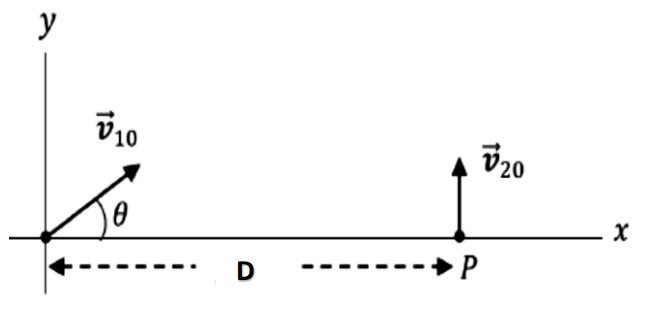
\includegraphics[width = 0.8\linewidth]{Figures/interception}
			\caption{Colisión de dos partículas en el aire}
			\label{fig:interception}
		\end{figure}
	
		
		\item \textbf{Escalera.} Una bola es lanzada por una escalera con velocidad inicial $\vec{v}_0$ con dirección horizontal, como se muestra en la figura \ref{fig:escalera}. Los escalones tienen altura $a$ y ancho $b = 2a$. Si la pelota golpea justo en la esquina derecha del segundo escalón, halle la altura $a$ en función de la velocidad y de la gravedad $g$.
		
		\begin{figure}[H]
			\centering
			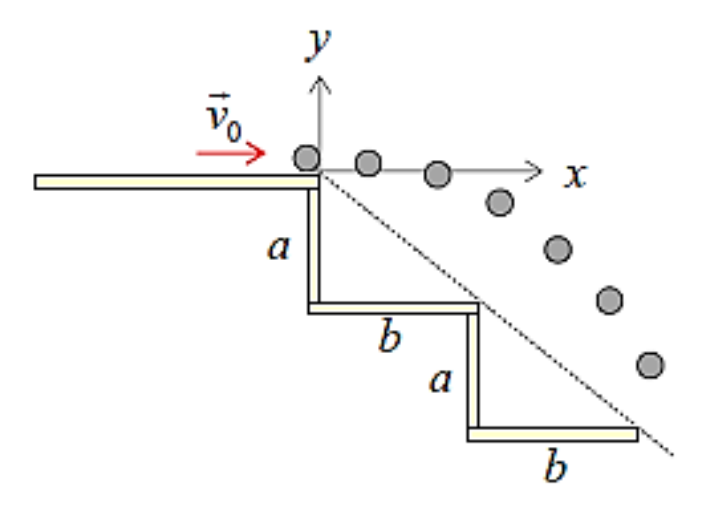
\includegraphics[width = 0.8\linewidth]{Figures/escalera}
			\caption{Bola en caída sobre una escalera}
			\label{fig:escalera}
		\end{figure}
		
		\item \textbf{Proyectil desde una avión.} Un avión baja en picada a una velocidad de $700 km/h$, formando un ángulo de $45^\circ$ con la horizontal. Cuando se encuentra a una altura de $400 m$ sobre el suelo, el avión suelta un proyectil. Calcular, a.) el tiempo que tarda el proyectil en llegar al suelo, b.) la velocidad con que llega y c.) el alcance del proyectil respecto al punto de lanzamiento.
		
		\item \textbf{Aceleración en coordenadas polares.} Muestre que la expresión de una aceleración $\vec{a}$ viene dada por 
		
		\begin{align*}
			\vec{a} = (\ddot{r} - r \dot{\theta}^2) \hat{r} + (r \ddot{\theta} + 2 \dot{r}\dot{\theta})\hat{\theta}
		\end{align*}
		
		Donde $\hat{r} = \cos \theta \hat{i} + \sin \theta \hat{j}$, y por tanto la posición de una partícula, a una distancia $r$ del origen del sistema de coordenadas y cuyo vector posición forma un ángulo $\theta$ con el eje $x$, viene dada por $\vec{r} = r \hat{r}$. El vector $\hat{\theta} = -\sin \theta \hat{i} + \cos \theta \hat{j}$.

		\item \textbf{Movimiento circular.} Demuestre que un movimiento circular (uniforme o no) la velocidad es perpendicular a la posición. Es decir que 

		\begin{align*}
			\vec{v}\cdot \vec{r} = 0
		\end{align*}

		y si además de ello es uniforme, 

		\begin{align*}
			\vec{v}\cdot\vec{a} = 0 && \vec{r} \cdot \vec{a} = -|\vec{a}||\vec{r}|
		\end{align*}

		\item \textbf{Ley de Kepler.} La segunda ley Kepler establece que los vectores posición de un planeta respecto al sol barre áreas iguales en tiempos iguales (véase la figura \ref{fig:kepler}). Hagamos un modelo ``naive'' y supongamos que los planetas se mueven únicamente en una trayectoria circular. La ley de gravitación de Newton establece que la fuerza gravitacional depende únicamente de la masa del planeta y el Sol, de la distancia entre ellos y tiene dirección radial. Bajo estas condiciones muestre que la ley de Kepler se cumple.
		
		\begin{figure}[H]
			\centering
			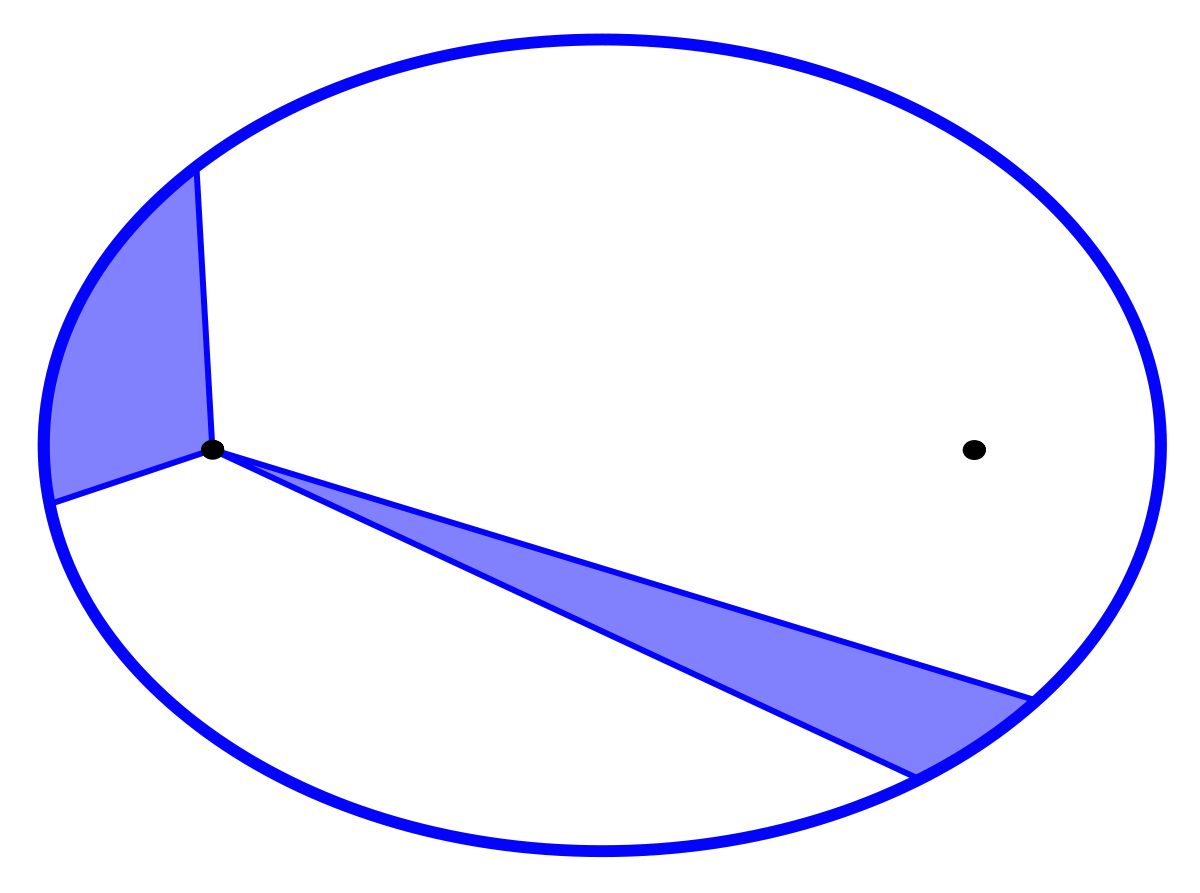
\includegraphics[width = 0.7\linewidth]{Figures/kepler}
			\caption{Segunda ley de Kepler-}
			\label{fig:kepler}
		\end{figure}
		
		% \item \textbf{Distancia a la Luna}. Suponga que la una se mueve alrededor de la Tierra en un movimiento circular uniforme, con periodo $T = 29.5 \text{ días}$. La aceleración que sufre la Luna debido a la fuerza gravitacional ($a_{Luna}$) viene dada por la ley de gravitación de Newton, que es 
		
		% \begin{align*}
		% 	a_{Luna} = G\frac{M_T}{r^2}
		% \end{align*}
		
		% Donde $G = 6.674 \times 10^{-11} \frac{N\cdot m^2}{kg^2}$ es la constante de gravitación universal, $M_T = 5.972 \times 10^{24} kg$ es la masa de la Tierra y $r$ es la distancia del centro de la Tierra al centro de la Luna. Sabiendo que el radio de la Tierra es $6371 km$, ¿cuál es la distancia más corta entre la superficie terrestre y el centro de la Luna?

		\item \textbf{Jerk.} La rata de cambio de la aceleración es conocida como ``jerk''. Encuentre la dirección y magnitud del jerk para una partícula que se mueve en un círculo de radio $R$ con velocidad angular $\omega$. Dibuje un diagrama mostrando los vectores de la posición, velocidad, aceleración y jerk.
		
		\item \textbf{Caminata sobre una rueda.} Una persona camina radialmente hacia fuera desde el centro de una plataforma circular con una rapidez constante de $0.1 m/s$. Simultáneamente, la plataforma rota desde el reposo con una aceleración angular de $0.1 rad/s^2$. El radio de la plataforma es de $2 m$. Calcular el tiempo y el número de vueltas que da la plataforma mientras la persona recorre la totalidad del radio.
		
		\item \textbf{Partícula en espiral.} Una partícula se mueve hacia afuera en una espiral. Su trayectoria es dada por $r=A\theta$, donde $A= (1/\pi)$ m/rad y $\theta$ aumenta en el tiempo deacuerdo a la ecuación $\theta = \alpha t^2/2$, donde $\alpha$ es una constante. a.) Haga un bosquejo del movimiento (puede usar un software si desea). b.) Muestre que la aceleración radial es cero cuando $\theta=1/\sqrt{2}$ rad. c.) \textquestiondown A qué ángulo la aceleración radial y tangencial tienen igual magnitud? 

		% \item \textbf{Espiral.} Una partícula se mueve en una trayectoria descrita por su posición radial dada por 
		
		% \begin{align*}
		% 	r(t) = r_0 e^{\omega t}
		% \end{align*}
		
		% Donde $r_0$ es la posición inicial y $\omega$ su velocidad angular constante. Calcular la velocidad y la aceleración de la partícula.
		
	\end{enumerate}
	
	\end{multicols}
\end{document}